%My thesis!
\documentclass[11pt,a4paper,titlepage]{report}
%\documentclass[a4paper,11pt,openright,twoside]{book}
\usepackage{amsmath}
\usepackage{ amssymb }
\usepackage{calligra}
\usepackage{amsfonts}
\usepackage[english]{babel}
\usepackage{verbatim}
\usepackage{indentfirst}
\usepackage{fancyhdr}
\usepackage{amsthm}
\usepackage{graphicx}
\usepackage{indentfirst}
\usepackage{microtype}
\usepackage{lmodern} 
\usepackage{braket}

\usepackage[font=small,labelfont=bf]{caption}  %per la didascalia delle immagini
\usepackage{mathrsfs}  %per fare le lettere calligrafiche
\usepackage{bm}  %per mettere le lettere greche in grassetto
\usepackage[T1]{fontenc}     %pacchetto lettere accentate
\usepackage[utf8]{inputenc}   %pacchetto lettere accentate

\newcommand{\HRule}{\rule{\linewidth}{0.5mm}}


\setlength\parindent{0pt}  % toglie identazione ovunque

% -----------------

\begin{document}

%--------------------------

\begin{titlepage}
%\begin{adjustwidth*}{10pt}{-40pt}
\begin{center}
\vspace*{-2.7cm}

\includegraphics{aquila_nome}
\\
\rule{\textwidth}{1pt}
\\[0.5cm]
{\Large DEPARTMENT OF MATHEMATICS}
\\[0.35cm]
{\Large MASTER DEGREE IN MATHEMATICS}
\\[2.3cm]
{\Large THESIS}
\\[1.5cm]
\textsc{\huge \textbf{Modeling and simulation of craniovertebral decompression}}
%\\[0.4cm]
%{\Large March 25th, 2015}
%\\[3cm]
\\[3cm]
\begin{minipage}{0.5\textwidth}
\flushleft {
\large Advisors: \\
 \textbf{Prof. Eleuterio F. Toro} \rule{0pt}{2.5ex}\\
 \normalsize University of Trento\\[0.4cm]
\large \textbf{Dr. Marie E. Rognes} \\
\large \textbf{Ms. Eleonora Piersanti} \\
 \normalsize Simula Research Laboratory\\[0.4cm] \rule{0pt}{2.5ex}}\\
\end{minipage}
\begin{minipage}{0.45\textwidth}
\flushright {\large
Student: \\
\rule{0pt}{2.5ex} \textbf{Carlo Cisale}\\
\normalsize University of Trento} \\
\end{minipage}

\vspace*{\fill}
{\Large ACADEMIC YEAR 2015-2016}
\rule{\textwidth}{1pt}


\end{center}
%\end{adjustwidth*}
\newpage
\thispagestyle{empty}
\phantom{}
\end{titlepage}
\newpage 
\thispagestyle{empty}

%--------------------------

\tableofcontents 
\pagenumbering{roman}

\newpage

\pagenumbering{arabic}

\chapter{Introduction}

\chapter{Medical background}

\chapter{Mathematical models}

\section{The Stokes Problem}
Let $\Omega$ be a unit square $[0,1]^2$, and let  $\partial \Omega_{inflow}$, $\partial \Omega_{outflow}$, $\partial \Omega_{sides}$ be, respectively, the top, bottom, and lateral boundaries. (PUT A PICTURE) \\
The strong formulation of the Stokes problem reads

\[
\begin{cases}
- \nabla \cdot (\nu \nabla u - pI) = f, & \mbox{in } \Omega \\
\nabla \cdot u = 0, & \mbox{in } \Omega
\end{cases}
\]

where we set Dirichlet boundary conditions as follows:

\[
\begin{cases}
u(x,y) = \left[ \begin{array}{c} 0 \\ x(1-x) \end{array} \right] , & \mbox{on } \partial \Omega_{inflow} \cup \partial \Omega_{outflow} \\

\vspace{.2cm}

u(x,y) = \left[ \begin{array}{c} 0 \\ 0 \end{array} \right], & \mbox{on } \partial \Omega_{sides}
\end{cases}
\]

In order to find a numerical solution to this problem, we write its variational formulation. Let $v$ be a test function in the space $\hat{V} = \set{u \in H^1(\Omega) | u_{|_{\partial \Omega}} = 0} $. Our aim is to find $(u(x,y),p(x,y)) \in V \times Q$ such that

\begin{align}
\int_\Omega -\nabla \cdot (\nu \nabla u - pI)v \,dx &= \int_\Omega fv \,dx, \\
\int_\Omega (\nabla \cdot u)q \,dx &= 0
\end{align}

Differentiating by part the right hand side of the first equation we obtain:

\begin{align}
\int_\Omega -\nabla \cdot (\nu \nabla u - pI)v \,dx &= \int_\Omega (\nu \nabla u - pI) \cdot \nabla v \,dx, \\
&- \int_{\partial \Omega} (\nu \nabla u - pI) \cdot n v \,ds.
\end{align}

Since we set Dirichlet boundary conditions on the entire boundary and $v_{|_{\partial \Omega}} = 0$, the boundary integral is zero. Hence, our weak formulation reads

\begin{align}
\int_\Omega (\nu \nabla u - pI) \cdot \nabla v \,dx &= \int_\Omega fv \,dx, \\
\int_\Omega (\nabla \cdot u) q \,dx &= 0.
\end{align}

Instead of using the space $V \times Q$, we use $V_h \times Q_h$, where $V_h$ and $Q_h$ are spaces defined with respect to a mesh $J_h$. We hence seek $(u_h, p_h) \in V_h \times Q_h$, where $V_h = \mathcal{P}^{cont,d}_{k+1} (J_h)$ and $Q_h = \mathcal{P}^{cont}_{k} (J_h)$ (typically we choose $k=1$). \\

As $u_h$ and $p_h$ are two approximate solutions, we want as well compute the errors

\begin{itemize}
\item $|| u_{exact} - u_h ||_{L^2}$,
\item $ | u_{exact} - u_h |_{H^1}$ (seminorm),
\item $|| p_{exact} - p_h ||_{L^2} $.
\end{itemize}

Since the pressure is defined up to some constant, we add the constraint 

\[
\frac{1}{|\Omega |} \int_{\Omega} p = 0,
\]

so we can compare an exact solution with mean value zero with the approximate solution. In order to do so, we can choose the following exact solutions:

\[
u_{exact} = \left[ \begin{array}{c} 0 \\ x(1-x) \end{array} \right], \quad 
p_{exact} = \frac{1}{2}-y.
\]

Using the previous solution, the error is 0, since the method for solving the problem is exact for polynomials, as shown below

%\begin{center}
%\begin{tabular}{| c | c |}
%\hline
%$|| u_{exact} - u_h ||_{L^2}$ & $4.9911 \times 10^{-14}$ \\
%\hline
%$ | u_{exact} - u_h |_{H^1}$ & $4.2006  \times 10^{-12}$ \\
%\hline
%$|| \nabla p_{exact} - \nabla p_h ||_{H^1} $ & $1.1943 \times 10^{-11}$ \\
%\hline
%\end{tabular}
%\end{center}

\begin{center}
\begin{tabular}{| c | c | c | c | c |}
\hline
$\mathbf{N}$ & $\mathbf{|| u_{exact} - u_h ||_{L^2}}$ & $ \mathbf{ | u_{exact} - u_h |_{H^1}}$ & $  \mathbf{|| p_{exact} - p_h ||_{H^1}} $ & $  \mathbf{ || p_{exact} - p_h ||_{L^2}}$ \\
\hline
$ 4 $ & $2.7373 \times 10^{-14}$ & $3.2162 \times 10^{-13}$ & $4.8674 \times 10^{-13}$ & $ 2.7373 \times 10^{-14}$ \\
\hline
$ 8$ & $1.3173  \times 10^{-12}$ & $7.5841 \times 10^{-11}$ & $1.4330 \times 10^{-10}$ & $ 1.3172  \times 10^{-12}$ \\
\hline
$ 16 $ & $ 8.4791 \times 10^{-14}$ & $9.1285 \times 10^{-12}$ & $3.5083 \times 10^{-11}$ & $ 8.4791 \times 10^{-14}$ \\
\hline
$ 32$ & $9.0508 \times 10^{-14}$ & $1.6039 \times 10^{-11}$ & $1.2406 \times 10^{-10}$ & $ 9.0580 \times 10^{-14}$ \\
\hline
$ 64$ & $6.3504 \times 10^{-13}$ & $9.5275 \times 10^{-11}$ & $1.4692 \times 10^{-9}$ & $ 6.3504 \times 10^{-13}$ \\
\hline
\end{tabular}
\end{center}


\newpage
A difference test case that could be used is:

\[
u_{exact} = \left[ \begin{array}{c} 0 \\ sin(\pi x) \end{array} \right], \quad 
p_{exact} = \frac{1}{2}-y.
\]

(Reminder: I put the $\pi$ in order for the exact solution to satisfy the boundary conditions!)
In the following tables, the convergence rate $k$ was computed as well, according to:

\[
k = \frac{log(\frac{E_{i+1}}{E_i})}{log(\frac{h_{i+1}}{h_i})}
\]

where we are assuming that $E_i \sim h^k_i$ and $E_{i+1} \sim h^k_{i+1}$. \\
The following table shows a second order convergence rate in $H^1$, as confirmed by the convergence plot.

\vspace{1cm}
\begin{figure}[ht]
\centering
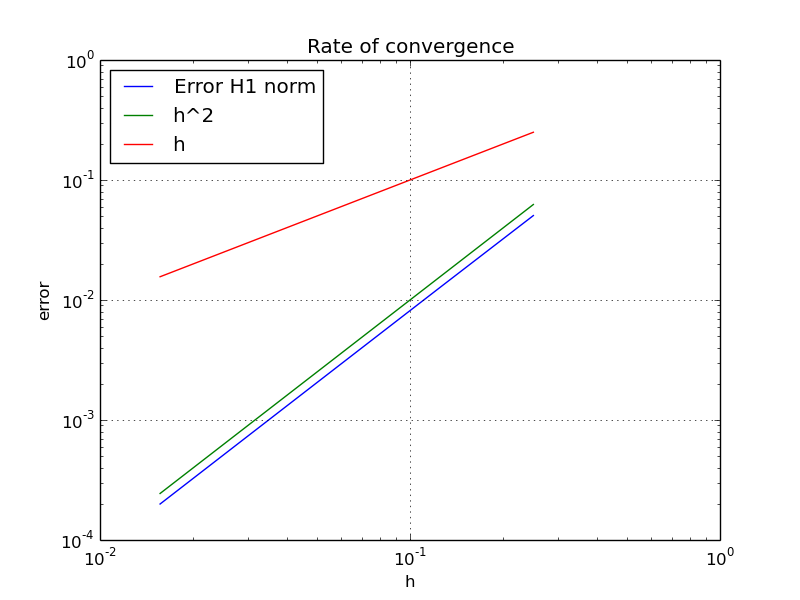
\includegraphics[width=\textwidth]{convergence_sine}
\caption{The plot shows a second order convergence, since the blue and green lines are parallel}
\end{figure}
\vspace{1cm}

\begin{center}
\begin{tabular}{| c | c | c | c | c |}
\hline
$  \mathbf{N}$ & $ \mathbf{|| u_{exact} - u_h ||_{L^2}}$ & $  \mathbf{ | u_{exact} - u_h |_{H^1}}$ & \textbf{Rate in }  $ \mathbf{H^1}$ & \textbf{Rate in } $  \mathbf{L^2}$  \\
\hline
$ 4 $ & $1.9388 \times 10^{-3}$ & $5.0548 \times 10^{-2}$  & & \\
\hline
$ 8$ & $2.4515  \times 10^{-4}$ & $1.2733 \times 10^{-2}$ &  $1.9890$ &  $2.9834$  \\
\hline
$ 16 $ & $ 3.0745 \times 10^{-5}$ & $3.1896 \times 10^{-3}$ & $1.9971$ & $ 2.9952 $  \\
\hline
$ 32$ & $3.8465 \times 10^{-6}$ & $7.9780 \times 10^{-4}$ & $ 1.9992 $ & $ 2.9987 $ \\
\hline
$ 64$ & $4.8092 \times 10^{-7}$ & $1.9948 \times 10^{-4}$ & $1.9998$ & $ 2.9997 $ \\
\hline
\end{tabular}
\end{center}



\begin{center}
\begin{tabular}{| c | c | c | c | c |}
\hline
$\mathbf{N}$ & $\mathbf{|| p_{exact} - p_h ||_{L^2}}$ & $\mathbf{|| p_{exact} - p_h ||_{H^1}} $ & \textbf{Rate in }  $ \mathbf{H^1}$ & \textbf{Rate in } $  \mathbf{L^2}$  \\
\hline
$ 4 $ & $1.4420  \times 10^{-4} $ & $ 1.3578  \times 10^{-3}$ & & \\
\hline
$ 8 $ & $ 1.1896  \times 10^{-5} $ & $ 2.2031 \times 10^{-4}$ & & \\
\hline
$ 16 $ & $ 1.0089  \times 10^{-6} $  & $ 3.7982 \times 10^{5}$ & & \\
\hline
$ 32 $ & $  8.7143 \times 10^{-8} $  & $ 6.6700 \times 10^{-6}$ & & \\
\hline
$ 64 $ & $ 8.0070 \times 10^{-9} $  & $ 1.1775 \times 10^{-6}$ & & \\
\hline
\end{tabular}
\end{center}


\section{The Navier-Stokes Equations on a fixed domain}
We now want to solve N-S equations. The problem reads: find the velocity $u(x,y,t)$ and the pressure $p(x,y,t)$ such that

\[
\begin{cases}
\rho \dot{u} + \rho (\nabla u \cdot u) - \nabla \cdot (\nu \nabla u - pI) = f, & \mbox{in } \Omega \\
\nabla \cdot u = 0, & \mbox{in } \Omega
\end{cases}
\]

As initial conditions (IC), we set $u(t=0) = u_0 = 0$. \\
As boundary conditions (BC), we use

\[
\begin{cases}
u(x,y,t) = u_{inflow}(x,y,t) , & \mbox{on } \partial \Omega_{top} \\
u(x,y,t) = u_{outflow}(x,y,t) , & \mbox{on } \partial \Omega_{bottom} \\
\sigma \cdot \vec{n} = 0,  & \mbox{on } \partial \Omega_{sides}
\end{cases}
\]

where $\sigma = \nu \nabla u - pI$, and for this example

\begin{equation}
u_{inflow} = u_{outflow} =  \left[ \begin{array}{c} 0 \\ x(x-1)sin(\pi \omega x) \end{array} \right].
\end{equation}

In order to solve this problem numerically using finite element method, we write its variational form. Let $v$ be a test function in

\[
\hat{V} = \set{v \in H^1(\Omega) | v_{|_{\partial \Omega_{top} \, \cup \, \partial \Omega_{bottom}}} = 0}
\]

and $q \in \hat{Q}$. Let us multiply the N-S equations by $v$ and $q$ and integrate on $\Omega$:

\begin{align}
&\int_{\Omega} \rho \, \dot{u} \, v \, dx + \int_{\Omega} \rho (\nabla u \cdot u)v \, dx - \int_{\Omega} \nabla \cdot (\nu \nabla u - pI)v \, dx = \int_{\Omega} fv \, dx \\
&\int_{\Omega} (\nabla \cdot u) q \, dx = 0.
\end{align}

I take the term $- \int_{\Omega} \nabla \cdot (\nu \nabla u - pI)v \, dx$, and integrate by parts:

\[
- \int_{\Omega} \nabla \cdot (\nu \nabla u - pI)v \, dx = \int_{\Omega} (\nu \nabla u - pI) \cdot \nabla v \, dx - \int_{\partial \Omega} (\nu \nabla u - pI) \cdot n \, v \, dx.
\]

The boundary term can actually be divided in three different terms (one for each part of the boundary), as $\partial \Omega = \partial \Omega_{top} \cup \partial \Omega_{bottom} \cup \partial \Omega_{sides}$. Since we chose $v \in \hat{V}$, the term on $\partial \Omega_{top} \cup \partial \Omega_{bottom}$ is zero. The term on $\partial \Omega_{sides}$ is also zero: since $\sigma = \nu \nabla u - pI$ and $\sigma \cdot \vec{n} = 0$ on $\partial \Omega_{sides}$, the remaining term on the boundary is also zero. Hence, $- \int_{\partial \Omega} (\nu \nabla u - pI) \cdot n \, v \, dx = 0$.

The variational form becomes

\begin{align}
&\int_{\Omega} \rho \, \dot{u} \, v \, dx + \int_{\Omega} \rho (\nabla u \cdot u)v \, dx - \int_{\Omega} (\nu \nabla u - pI \cdot \nabla v \, dx = \int_{\Omega} fv \, dx \\
&\int_{\Omega} (\nabla \cdot u) q \, dx = 0.
\end{align}

\subsection{Time discretization}
We now want to use a Crank-Nicolson discretization (second order in time) of the N-S equations: let $[0, T] = \cup^N_{i=0} [t_i, t_{i+1}] $ be the time interval, and $\Delta t$ the time step. \\
Let $u^i$ be an approximation of $u(t_i)$. We want to compute $u^{i+1}$ and $p^{i+1}$, i.e. an approximation of $u$ and $p$ respectively at the time level $t_{i+1}$, hence $u^{i+1} \approx u(t^{i+1})$ and $p^{i+1} \approx p(t^{i+1})$. \\
The Crank-Nicolson discretization reads:

\[
\left\{  
\begin{aligned}
& \rho \frac{u^{i+1} - u^i}{\Delta t} + \rho (\nabla u^{mid} \cdot u^i) - \nabla \cdot (\nu \Delta u^{mid} - p^{mid}I) = f^{mid} \\
& \nabla u^{i+1} = 0
\end{aligned}
\right.
\]

where we set $u^{mid} = \frac{u^i + u^{i+1}}{2}$.

\subsection{Spatial discretization}
We multiply the Navier-Stokes equations, respectively, by the test functions $v$ and $q$. We choose $v \in \hat{V} = \set{v \in [H^1(\Omega)]^2 | v_|{_{\partial \Omega_{top} \cup \Omega_{bottom}}} = 0}$, and $q \in \hat{Q}$ (SPECIFY $\hat{Q}$). \\
Problem: find $(u^{i+1}, p^{i+1}) \in \hat{V} \times \hat{Q}$ such that 

\[
\left\{  
\begin{aligned}
& \langle \rho \frac{u^{i+1} - u^i}{\Delta t},v \rangle_\Omega
+ \langle \rho \nabla u^{mid} \cdot u^i  ,v \rangle_\Omega
- \langle v \nabla \cdot (\nabla u^{mid}) ,v \rangle_\Omega
+ \langle \nabla p^{mid} ,v \rangle_\Omega = \langle f^{mid} ,v \rangle_\Omega \\
& \langle \nabla \cdot u^{i+1},v \rangle_\Omega.
\end{aligned}
\right.
\]

for all $(v,q) \in V \times Q$.

Since the boundary term in (PUT REFERENCE) is always zero, the following holds:

\[
\begin{aligned}
\langle \nabla \cdot (\nu \nabla u - pI) ,v \rangle_\Omega & = \langle \nu \nabla u - pI ,\nabla v \rangle_\Omega \\
														& = \langle \nu \nabla u  ,\nabla v \rangle  - \langle p ,\nabla \cdot v \rangle_\Omega										
\end{aligned}
\]

Hence we obtain:

\[
- \langle \nabla \cdot (\nu \nabla u^{mid} - p^{mid}I) ,v \rangle_{\Omega} = \langle \nu \nabla u^{mid}, \nabla v \rangle_\Omega -  \langle p^{mid}, \nabla \cdot v \rangle_\Omega.
\]

So the numerical scheme reads:

\[
\left\{  
\begin{aligned}
& \langle \rho \frac{u^{i+1} - u^i}{\Delta t},v \rangle_\Omega
+ \langle \rho \nabla u^{mid} \cdot u^i  ,v \rangle_\Omega
+ \langle \nu \nabla u^{mid}, \nabla v \rangle_\Omega
- \langle p^{mid} , \nabla \cdot v \rangle_\Omega = \langle f^{mid} ,v \rangle_\Omega \\
& \langle \nabla \cdot u^{i+1},v \rangle_\Omega.
\end{aligned}
\right.
\]

and then

\[
\left\{  
\begin{aligned}
\rho \langle u^{i+1},v \rangle_\Omega - \rho \langle u^i, v \rangle_\Omega & + \Delta t \rho \langle \nabla u^{mid} \cdot u^i  ,v \rangle_\Omega \\
& + \Delta t \nu \langle \nabla u^{mid}, \nabla v \rangle_\Omega \\
& - \Delta t \langle p^{mid} , \nabla \cdot v \rangle_\Omega \\
& = \Delta t \langle f^{mid} ,v \rangle_\Omega \\
\langle \nabla \cdot u^{i+1},v \rangle_\Omega.
\end{aligned}
\right.
\]

Instead of using the space $V \times Q$, we use $V_h \times Q_h$, where $V_h$ and $Q_h$ are spaces defined with respect to a mesh $J_h$. We hence seek $(u_h, p_h) \in V_h \times Q_h$, where $V_h = \mathcal{P}^{cont,d}_{k+1} (J_h)$ and $Q_h = \mathcal{P}^{cont}_{k} (J_h)$ (typically we choose $k=1$). \\

\section{Navier-Stokes on a moving domain}

\section{Navier-Stokes on a moving domain where the movement depends on $(u,p)$}

\chapter{Numerical methods}

\section{Finite element formulation}
\section{FEniCS}
\section{Numerical schemes}

\chapter{Verification/Validation}

\section{Stokes}
\section{Channel flow}
\section{Driven cavity}
\section{ALE test case}
See Vegard
\section{ALE + elasticity test case}

\chapter{Numerical results}

\chapter{Discussion}

\chapter{Conclusions}

\end{document}